\documentclass{aicom2e}
\usepackage{amsmath}
\interdisplaylinepenalty=2500
\usepackage[algo2e,ruled,vlined,linesnumbered]{algorithm2e}
\usepackage[active]{srcltx}


\usepackage{amsthm, amssymb,amsfonts}
\usepackage{graphicx}
\usepackage{epsfig}
\usepackage{latexsym}
\usepackage{colortbl}
\usepackage{times}
\usepackage{helvet}
\usepackage{courier}
\usepackage{caption}
\usepackage{subfig}
\usepackage{float}
\usepackage{xcolor}
\usepackage{pslatex}
\usepackage{eso-pic}
\usepackage[bottom]{footmisc}
\usepackage{url}
\usepackage{etex}


\newtheorem{definition}{Definition}
\newtheorem{lemma}{Lemma}
\newtheorem{theorem}{Theorem}
\newtheorem{observation}{Observation}
\newcommand{\kgs}{$k$-goal search}
\newcommand{\kgbfs}{$k$-goal best-first search}


\newcommand{\astar}{A$^*$}
\newcommand{\kastar}{kA$^*$}
\newcommand{\minf}{Min-f}
\newcommand{\maxf}{Max-f}
\newcommand{\tuple}[1]{\ensuremath{\left \langle #1 \right \rangle }}
\newcommand{\open}{\textsc{Open}}
\newcommand{\closed}{\textsc{Closed}}
\DeclareMathOperator*{\argmin}{\arg\!\min}
\newcommand{\roni}[1]{\textbf{[RS:#1]}}
%\newenvironment{proof}{\noindent{\bf Proof:~~}}{\qed}

\begin{document}
\begin{frontmatter}                           % The preamble begins here.
%
%\pretitle{Pretitle}
\title{Shortest Path for K Goals}
% \runningtitle{Running title}
%\subtitle{Subtitle}
\maketitle
%
\author[]{Meir Goldenberg}
\address{The Jerusalem College of Technology\\ Jerusalem, Israel\\
	E-mail: mgoldenbe@gmail.com}
\author[]{Roni Stern}
\address{Ben Gurion University of the Negev\\ Be'er Sheva, Israel\\
E-mail: roni.stern@gmail.com}
\author[]{Ariel Felner}
\address{Ben Gurion University of the Negev\\ Be'er Sheva, Israel\\
	E-mail: felner@bgu.ac.il}

\begin{abstract}
Abstract...

\end{abstract}

\begin{keyword}
artificial intelligence\sep AI\sep Heuristic Search
\end{keyword}
%
\end{frontmatter}

\section*{Introduction}


The shortest path problem (SSP) in a graph is the problem of finding the lowest cost path in a graph from one vertex -- denoted the {\em start} vertex -- to another vertex -- denoted the {\em goal} vertex. 
SSP is a well-studied problem and many algorithms have been proposed for solving it. 

Now, imagine $k$ SSP problems, such that all the problems share the same start vertex. 
Solving this set of SSP problems is called the $k$-goal problem. 
A trivial solution to \kgs\ is to run a SSP solver $k$ times. Alternatively, 
we can construct a $k$-dimensional SSP problem, and try to solve all the $k$ SSP problems concurrently. 
In this work we study the interplay between these two extreme approaches and
study how heuristics can be used correctly to solve \kgs. 


\roni{TODO: SOME RELATED WORK?}

\section{Background and Problem Definition}

%In this section, we formally define the $k$-goal search problem.

% Graphs, costs, SSP
Let $G=(V,E,w)$ be a weighted graph, where $w:E\rightarrow \mathbb{R}^+$ is a function that assigns a non-negative real value for every edge. This value is referred to as the {\em cost} of the edge and the cost of a path in a graph is  the sum the edge costs along it. 
In the Artificial Intelligence literature, graphs are often used to represent state spaces, 
where the graph vertices represent possible states of the world, the out-going edges of a vertex represent possible actions that an agent can perform in the corresponding state, and the cost of that edge represents the cost of the corresponding action. 
Thus, throughout this paper we will use the terms {\em states} and {\em actions} instead of vertices and edges, respectively, and use the term {\em applying an action} instead of traversing an edge. Note that a path in a graph corresponds to an applicable sequence of actions. 

\begin{definition}[The Shortest Path Problem (SPP)]
A shortest path problem (SPP) is defined by a tuple $\tuple{G,s, g}$, 
where $s$ and $g$ are states in $G$ and the problem is to find the lowest cost path in $G$ from $s$ to $g$. 
\end{definition}

\subsection{The \astar{} Algorithm}




\begin{algorithm2e}[t!]
	\small
	\KwIn{Start state $s$, Goal state $g$)}
	$g(s)\gets 0$; \open{}~$\gets\emptyset$; \closed{}~$\gets \emptyset$\\
	Add $s$ to \open{} with $f(s)=g(s)+h(s)$\\
	\While {\open{} $\neq \emptyset$} {
		$n \gets \argmin\limits_{n\in\open{}} f(n)$ \nllabel{line:open:chooseNode}\\
		Move $n$ from \open{} to \closed{}\\
		\lIf {$n$ is the goal state}{\Return $n$}
		\For{every action $a$ applicable at state $n$ \nllabel{line:nextNeighbor}}{
			$c \gets $ generate a state by applying $a$ to $n$ \nllabel{line:astar:generate-start}\\			
			
			% Duplicate detection
			\If{$c$ in $\open{}\cup \closed{}$ \nllabel{line:dd-start}}{
				\If{$g(c) \leq g(n)+w((n,c))$}{
					Continue (goto line~\ref{line:nextNeighbor})
				}
				Remove $n$ from \open{} and \closed{}  \nllabel{line:dd-end}\\
			}
			% Update n's g and f values
			$g(c)\gets g(n)+w((n,c))$ \nllabel{line:compute-f}\\ 							
			Add $c$ to \open{} with $f(c)=g(c)+h(c)$  \nllabel{line:astar:generate-end}\\
		}
	}
	\Return No solution exists\\ 
	\caption{\astar{}}
	\label{alg:astar}
\end{algorithm2e}



% A* for single agent search
SPP has been well-studied in the literature. \astar{}~\cite{hartNR68Astar} is a popular 
heuristic search algorithm for solving SPP. For completeness, we provide below a short description of the \astar{} algorithm (see Algorithm~\ref{alg:astar} for the pseudo code of \astar{}). 
\astar{} maintains two lists of states: \open{} and \closed{}. 
Initially, \closed{} is empty and \open{} contains only the start state. 
Every state that is added to \open{} is associated with a $g$ value and an $f$ value. 
The $g$ value of a node $n$, denoted $g(n)$, is the cost of the lowest cost path found so far from the start state $s$ to $n$, where $g(s)$ is set to zero. 
The $f$ value of $n$, denoted $f(n)$ is the sum of $g(n)$ and a heuristic estimate of the cost of the lowest cost path from $n$ to the goal state $g$. 
This heuristic estimate is denoted by $h(n)$, and there is an abundance of prior work in the literature on how to develop effective heuristics. \roni{TODO: Add some refs here}


In every iteration of the classical \astar{} algorithm, the state with the lowest $f$ value in \open{} is moved from \open{} to \closed{}. 
If that node is a goal, the search halts. Otherwise, the state is {\em expanded}.  
Expanding a state $n$ means generating every state that can be reached by applying a single action at state $n$. 
Then, the $g$ and $f$ values of every generated state $c$ are computed based on the $g$ value of its parent, the cost of the action used to generate $c$, and the heuristic estimate $h(c)$. Finally, the generated nodes are added to \open{} with their $f$ values, to be considered for expansion in future iterations. Since the searched graph may not be a tree, multiple paths to the same state may be explored, and \astar{} keeps track of only the best (lowest cost) path it finds to every generated state (lines~\ref{line:dd-start}-\ref{line:dd-end}).  


\roni{TODO: Maybe add more line numbers to the text?}
\roni{TODO: Add something on tie breaking}

% A* properties and admissible heursitics
\astar{} has several important properties. First, if the heuristic used is {\em admissible}, i.e., it does not over-estimate the cost of the lowest cost path to the goal, then \astar{} is guaranteed to solve SPP, i.e., to return a lowest cost path from $s$ to $g$.\footnote{In fact, it is sufficient that the heuristic will be admissible only on states that are on a single lowest-cost path for \astar{} to guarantee optimality.} 
Second, if the heuristic is {\em consistent} then \astar{} is guaranteed to never expand a state more than once. 
%when a state $n$ is expanded it is guaranteed that the lowest cost path from $s$ to $n$ has been found, and thus $g(n)$ is the cost lowest cost path from $s$ to $n$. 
\begin{definition}[Consistent Heuristic]
	A heuristic $h$ is consistent if for every pair of states $n$ and $c$ such that expanding $n$ generates $c$ 
	it holds that 
	\[ h(n)\leq w((n,c))+h(c) \]
	\label{def:consistent}
\end{definition}
%The important implication of a consistent heuristic is that \astar{} with a consistent heuristic is guaranteed to expand every state at most once. 
Third, under some conditions it can be shown that, up to tie-breaking between states with equal $f$ values, \astar{} will only expand the minimal set of states required to find an optimal solution~\cite{dechter1985generalizedBestFirst}. 
A recent generalization of \astar{} provides a similar guarantee with respect to the number of states generated as well~\cite{goldenberg2014enhanced}. This type of guarantees, often referred to as the {\em optimally effective} property of \astar{}, is  important because in many cases the runtime of the algorithm is correlated with the number of states expanded/generated. 
Thus, guaranteeing that \astar{} expands the minimal number of states provides some sort of optimality guarantee for \astar{}'s efficiency compared to equally informed algorithms. 



\subsection{The $k$-Goal Problem}
In this paper we focus on the $k$-goal search problem, which can be viewed as a generalization of SPP. 

\begin{definition}[$k$-goal search]
	A \kgs\ problem is defined by a tuple $\tuple{G,s, g_1, g_2, \ldots, g_k}$, 
	where $s$ and $g_1, g_2, \ldots, g_k$ are states in $G$ and the problem is to find 
	$k$ paths $p_1,\ldots p_k$ such that for every $i\in [1,k]$ it holds that $p_i$ is a lowest-cost path from $s$ to $g_i$. 
\end{definition}


% k searches independentaly
Clearly, SPP is a special case of \kgs\ with $k=1$. A trivial solution to the \kgs\ problem is to consider it as $k$ independent SPPs and use a SPP algorithm such as \astar{} to solve these problems. In the next section we present this approach and analyze its complexity. 
In later sections we explore a different approach to solving the \kgs\ problem that considers \kgs{} as a single search problem, in an effort to re-use information between the $k$ tasks. 




\section{$k$ Searches for One Goal}

\begin{algorithm2e}[t!]
	\small
	\KwIn{Start state $s$, Goal states $g_1,\ldots g_k$)}
	\For{$i$=1 to $k$}{
		$p_i\gets$ \astar{}($s$,$g_i$)\\
	}
	\Return $p_1,\ldots p_k$\\	
	\caption{Solving \kgs{} with $k$ \astar{}s}
	\label{alg:k-searches}
\end{algorithm2e}

Algorithm~\ref{alg:k-searches} outlines the trivial approach for solving \kgs{}: running \astar{} $k$ times, where every run solves the SPP for one of the $k$ goals. The resulting $k$ paths are returned as a solution to the \kgs{} problem. 
To analyze the effectiveness of approach, we use the notions of {\em necessary} states and {surplus} states~\cite{goldenberg2014enhanced}. 
\roni{Meir and Ariel: who used this term before us?}

\begin{definition}[Surplus States and Necessary States]
	Let $\Pi$ be a SPP defined by the tuple $\tuple{G,s,g}$, and let $opt_\Pi$ denote the cost of a solution to $\Pi$. 
	A state $n$ is called a {\bf necessary} state with respect to $\Pi$ if $f(n)<opt_\Pi$. 
	A state $n$ is called a {\bf surplus} state with respect to $\Pi$ if $f(n)>opt_\Pi$. 
\end{definition}
Without any additional knowledge of the graph $G$, one needs to expand every necessary state in order to solve a given SPP, 
and one can solve a given SPP without expanding any surplus state. \roni{Meir/Ariel, what would be a good reference to put here? Dechter and Pearl? it is important to be accurate here}
\astar{} is guaranteed to expand all necessary nodes and not a single surplus node. Consequently, 
using Algorithm~\ref{alg:k-searches} to solve a \kgs{} problem will end up expanding all the necessary states 
for finding the required $k$ shortests path, without expanding any surplus state. 
In plainer words, it seems that Algorithm~\ref{alg:k-searches} is ``optimally effective'' for \kgs{}, 
expanding exactly the set of needs one must expand in order to solve the problem, up to tie-breaking between states with the same $f$ value. 


This conclusion, however, is not accurate, as it overlooks two potential sources for improvement:
\begin{itemize}
	\item {\bf Learning from experience.} When solving one SPP problem, e.g., for goal $g_1$, one gains additional knowledge of the searched graph, which may be used when solving the subsequent SPPs for the other goals.
	\item {\bf Avoiding duplication.} The same state can be generated and expanded in multiple SPPs. For example, using Algorithm~\ref{alg:k-searches} will end up generating the children of the start state at least $k$ times. This introduces redundancy to the search process that may be avoided.  
\end{itemize}
The first source of improvement is closely related to the literature on incremental search and to moving-target search algorithms. Thus, we focus on this work on the latter source of improvement -- avoiding redundancy in the search process. 
\roni{Meir and Ariel: the above paragraph is a potential mine (as Ariel likes to call them). But on the other hand, I think it is correct. Let me know what you think, and also, help me in adding appropriate references.}
Next, we analyze these redundancies. 

\subsection{Redundancies in the $k$ Searches Approach}

To analyze the redundant operations performed by the $k$ search approach, we first describe the operations performed by \astar{} whenever a state is generated (lines~\ref{line:astar:generate-start}-\ref{line:astar:generate-end} in Algorithm~\ref{alg:astar}):
\begin{enumerate}
\item {\bf Generation}  (line~\ref{line:astar:generate-start}). This means computing the generated state by applying 
an action to the expanded state. This step usually involves setting up some data structure that represents the generated state. If the action generating the state is not too complicate, the complexity of this step is linear in the size of the state. 
\item {\bf Duplicate detection}  (lines~\ref{line:dd-start}-\ref{line:dd-end}). This means performing a lookup in \open{} and \closed{} to see if the generated state was already generated, and if so, whether the current path to it is better than the one previously found. The lookup in \open{} and \closed{} is often implemented by storing all the nodes that were generated in the past in some hash table and performing an $O(1)$ hash table lookup. We denote the computational cost of this step as $C_{dd}$. 
\item {\bf Heuristic computation}  (line~\ref{line:compute-f}). This means computing the $h$ value of the generated node. Heuristics vary widely in their computational cost, where some heuristics require constant time to compute while more sophisticated heuristics may involve poly-time computations. We denote the computational cost of this step as $C_{h}$. 
\item {\bf Insertion into \open{}}  (line~\ref{line:astar:generate-end}). This means adding a state to \open{} with an associated $f$ value. \open{} are often implemented as a Binary heap or priority queue sorted according to $f$ values, so that extracting the state with lowest $f$ value is very fast. Thus, inserting a state to \open{} may take time that is logarithmic in the size of \open{}. We denote the computational cost of this step as $C_{add}$.  
\end{enumerate}
Each of these operations incur some computational cost. Let $C_{gen}, C_{dd}, C_{h},$ and $C_{add}$ denote the average computation cost 
of the above four operations, generation, duplicate detection, heuristic computation, and insertion into \open{}, respectively, 
and let $Gen(g_i)$ denote the set of nodes generated by \astar{} when it is used to solve SPP for goal $g_i$.  
Clearly, the $k$ searches approach incurs at least $\sum_{i=0}^k C_{gen}+C_{dd}+C_{h}+C_{add}$ in terms of computation cost, 
even if when the states generated by these searches are almost the same. 

\begin{figure}
	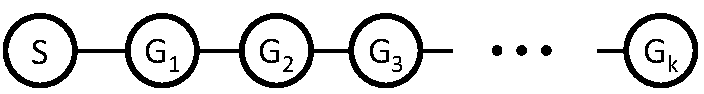
\includegraphics[width=\columnwidth]{k-search-bad_cropped}
	\caption{An example where the $k$ search approach is inefficient.}
	\label{fig:k-search-bad}
\end{figure}
An extreme example of this inefficiency is depicted in Figure~\ref{fig:k-search-bad}. The searched graph is a simple line, 
where $g_1$ is adjacent to $s$, $g_2$ is adjacent to $g_1$, and so on. In this case the $k$ searches approach would generate
$1+2+3+\cdots+k=\frac{k(k-1)}{2}$ while it is easy to see that generating $k$ states would be sufficient to solve the \kgs{} for this case. 


% Some costs can be saved
More generally, consider the costs incurred when generating a state $n$ for more than one goal. 
The costs incurred for heuristic computation ($C_{h}$) may be unavoidable. This is because to prove that a path of cost $X$ to a goal $g_i$ is optimal one needs to expand all the necessary nodes, i.e., generate their children and compute their $f$ values. This is needed to verify that all paths of costs smaller than $X$ have been considered. Since the $f$ value of a state may be different when searching for different goals, this means that a state may be necessary for one search and not necessary for the other. 
Thus, the search must check that $n$ is necessary for each goal independently, incurring a computational cost of $C_{h}$ per goal. 



However, when a state is generated by more than one search there is potential for saving some of the computational costs incurred during its generation. In particular, by generating such states only once, one may save the costs incurred for node generation, duplicate detection, and insertion to \open{} ($C_{gen}, C_{dd},$ and $C_{add}$). In the next section we propose a method for doing so. 



\section{One Search for $k$ Goals}
In this section we generalize \astar{} to search for $k$ goals in parallel. 
We call the resulting algorithm \kastar{}. 
Before presenting a complete pseudo code for \kastar{}, we highlight several differences it has from \astar{}. 

\subsubsection*{Multiple heuristics per state.} When a state $n$ is generated, \kastar{} computes 
$k$ different $h$ values for it $h_1(n),\ldots h_k(n)$, such that $h_i(n)$ is the heuristic estimate of the cost to get from $n$ to goal $G_i$. These $k$ heuristic values are used to compute $k$ different $f$ values $f_1(n),\ldots f_k(n)$, such that $f_i(n)=g(n)+h_i(n)$. We discuss later how \open{} is prioritized with respect to these $k$ values, and refer to this value for now as $F_n$. Note that computing $F_n$ costs $k\cdot C_h$, and thus the computation cost of generating a state in \kastar{} is larger than that of \astar{} by $(k-1)\cdot C_{h}$.\footnote{As dicsussed later in the paper, the actual computational cost in \kastar{} can be smaller, since as the search progresses the list of relevant goals becomes smaller, and consequently computing $F_n$ becomes easier.}

\subsubsection*{Maintaining the relevant goals.} In \astar{} when a goal is expanded the search halts. By contrast, in \kastar{} the search does not halt until a lowest-cost path to each of the $k$ goals is found. To this end, \kastar{} tracks of the set of goals that were not solved yet, i.e., the goals where the lowest cost path to them has not been found. This set of goals is referred to as the {\em relevant goals}. Maintaining the list of relevant goals is also used to avoid redundant heuristic computations: when a state is generated we only compute the heuristics for goals that are still relevant. 



%\subsubsection*{Node evaluation function.} When searching for a single lowest-cost path with \astar{}, the nodes are popped from \open{} according to their $f=g+h$ values. In \kastar{}, we compute the $h$-value forand associate every node in \open{} with a value that considers the $h$-value for each of the $k$ goals.     Thus, when a node is generated then we compute the heuristic for each of the $k$ goals.




\begin{algorithm2e}[t!]
	\KwIn{Start state $s$, goal states $G_1,\ldots,G_k$}
	%\SetKwBlock{KGBFS}{$k$-goal best-first-search(start state $s$, goal states $G_1,\ldots,G_k$)}
	\open{}~$\gets\emptyset$ \\
	{\tt RelevantGoals} $\gets \{G_1,\ldots,G_k\}$ \nllabel{line:init-relevant-goals} \\
	$F_s\gets$ ComputeF(s, RelevantGoals) \nllabel{line:compute-f-start}\\
	Add $s$ to \open{} with key $F_s$ \\		
	\While {\open{} $\neq \emptyset$ and {\tt RelevantGoals} not empty} {
		$best \gets$ node in $\open{}$ with the smallest key \nllabel{line:open:chooseNode}\\
		Remove $best$ from \open{}\\
		\If {$best\in$ {\tt RelevantGoals}}{
			Add path to $best$ to the solution \nllabel{line:storePath}\\
			Remove $best$ from {\tt RelevantGoals} \nllabel{line:removeGoal}\\
		}
		\For{$n \in neighbors(best)$}{
			$F_n\gets$ ComputeF(n, {\tt RelevantGoals})\\
			Add $n$ to \open{} with key $F_n$ \\
		}
	}
	\caption{\kastar{}}
	\label{alg:k-goal-bfs}
\end{algorithm2e}



Algorithm~\ref{alg:k-goal-bfs} shows the pseudo code for \kastar{}. Initially, all goals are inserted into the list of relevant goals ({\tt RelevantGoals}) [line~\ref{line:init-relevant-goals} in Alg.~\ref{alg:k-goal-bfs}]. The initial state is inserted into \open{} [line~\ref{line:compute-f-start}], associated with . 
Every node $n$ that is added to \open{} is associated with a key value $F_n$ that is computed using the {\tt ComputeF} function. In every iteration, the node with the smallest key value is popped out of \open{} (line~\ref{line:open:chooseNode}). If it is a goal then we store the path to it (line~\ref{line:storePath}). In addition, we remove that goal from the {\tt RelevantGoals} list, to mark that we are no longer looking for a path to that goal (line~\ref{line:removeGoal}). When the {\tt RelevantGoals} list is empty, we halt the search, having found a path to each goal. 


It is easy to see that Algorithm~\ref{alg:k-goal-bfs} is complete and sound, in the sense that if there are paths to the $k$-goals they will be found, and the paths returned by the algorithm are all valid paths to the $k$ goals. The key question is whether these paths are indeed the optimal path to the $k$-goals.
As we show next, this depends on the order according to which nodes are expanded, 
which in turn depends on how $F_n$ is computed. %)the {\tt ComputeF} function is implemented. 


\subsection{An Evaluation Function for \kastar{}}
In \astar{} for a single goal, states are prioritized in \open{} according to the $f=g+h$ value of a node. 
In contrast, a state in \kastar{} has $k$ heuristic values ($h_1(n),\ldots,h_k(n)$) and 
consequently $k$ $f$ values ($f_1(n),\ldots,f_k(n)$) one per goal. Therefore, \kastar{} requires a node evaluation function that aggregates these $f$ values in some way. In Algorithm~\ref{alg:k-goal-bfs} this is encapsulated in the {\tt ComputeF} function. We refer to the value returned by this function as the state's $F$ value, and consider the following two options for computing it. 
\begin{align}
F_{min}(n)=&\min_{i\in [1,k]}f_i(n) & (\textbf{\minf})\\ 
F_{max}(n)=&\max_{i\in [1,k]}f_i(n) & (\textbf{\maxf})\\ 
\end{align}


%\subsection{$F_{min}$}

\begin{theorem}[\minf{} is admissible]
If $h$ is an admissible heuristic, then running \kastar{} with $F_{min}$ 
as the node evaluation function ({\tt ComputeF}) will return $k$ paths $\pi_1,\ldots, \pi_k$ such for every $i$ we have that $\pi_i$ is a lowest cost path from $s$ to $G_i$. 
\label{the:min-f}
\end{theorem}
 \begin{proof}
To prove this, we show that when a goal node is expanded for the first time, then its $g$ value is guaranteed to 
be the cost of the lowest-cost path from $s$ to that goal. 
By negation, assume that a goal $G_i$ was expanded, but there is a better path to $G_i$
that has not yet been discovered. Since \kastar{} is a best-first search, \open{} has some node $n$ that is on a better path to $G_i$ and has not been expanded yet. 
That is, 
\begin{equation}
g(n)+h_i(n)<g(G_i)
\label{eq:proof-1}
\end{equation}
Since $G_i$ was chosen to be expanded before $n$, it must have a $F_{min}$ value no-larger than $n$, i.e.,
\begin{align}
F_{min}(n) &\geq  F_{min}(G_i)\\
g(n)+\min_j h_j(n)& \geq  g(G_i)+\min_{j'} h_j(G_i)\\
g(n)+\min_j h_j(n)& \geq  g(G_i)\\
g(n)+h_i(n) &\geq  g(G_i) 
\end{align}
The last line above exactly contradicts Equation~\ref{eq:proof-1}. 
\end{proof}


%\subsection{$F_{max}$}
 
 \begin{figure}
 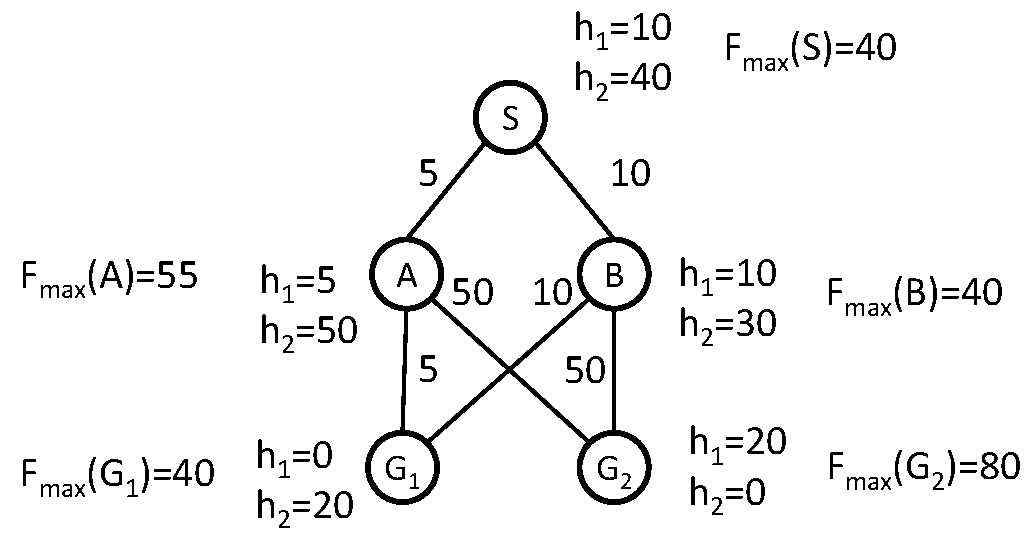
\includegraphics[width=\columnwidth]{max-bad_cropped.pdf}      
 \caption{An example of where using Max-$f$ returns a non-optimal solution. In this example, 
 using Max-$f$ will results in the following expansion order: $S$, $B$, $G_1$. 
 Thus, when $G_1$ is expanded, the best path known to it costs 25, while a 
 better path to it goes through $A$ and costs only 10.}
 \label{fig:max-bad}
 \end{figure}
 
 \begin{observation}[\maxf{} is not admissible]
 	Even if $h$ is an admissible heuristic, 
 	running \kastar{} with $F_{max}$ 
 	as the node evaluation function ({\tt ComputeF}) may return a path $\pi_i$ from $s$ to $G_i$ that is not optimal. 
 	\label{obs:max-f-inadmissible}
 \end{observation}
To demonstrate Observation~\ref{obs:max-f-inadmissible}, consider the graph in Figure~\ref{fig:max-bad}.
 In this example, using \maxf{} will result in the following expansion order: $S$, $B$, and then $G_1$. At this stage, we expanded one of the goals -- $G_1$ -- while the best path found so far to it goes through $B$ and costs 40. However, a better path to it is through $A$, which costs only 10.
 
 
 % MAX-F is OK for consistent heuristics
  The observant reader may have noticed that the heuristic function in Figure~\ref{fig:max-bad} is inconsistent (Definition~\ref{def:consistent}): $h_2(A)=50$ while its child, $G_1$, which is connected to it via an edge of cost 5, has $h_2(G_1)=20$. If $h$ was consistent the $h_2(A)-c(A,G_1)\leq h_2(G_1)$, where e$c(A,G_1)$ is the cost of the edge between $A$ and $G_1$. 
  Interestingly, if the heuristic used is consistent then using \maxf{} in \kastar{} is possible, guaranteeing that all paths returned are optimal. % wi(Definition~\ref{def:consistent}), then \maxf{} is admissible for \kastar{}. %the inadmissibility of Max-$f$ is related to the {\em inconsistency} of the used heuristic. 
 
 
\begin{theorem}[\maxf{} is admissible if $h$ is consistent]
If $G$ is undirected and $h$ is admissible and consistent, 
then running \kastar{} with $F_{max}$ 
as the node evaluation function ({\tt ComputeF}) 
will return $k$ paths $\pi_1,\ldots, \pi_k$ such for every $i$ we have that $\pi_i$ is a lowest cost path from $s$ to $G_i$. 
\label{the:max-f}
\end{theorem}
 \begin{proof}
 Assume by negation that Theorem~\ref{the:max-f} is not correct. This means
 that there is a case where a goal $G_i$ is expanded while $g(G_i)$ is not optimal. Since \kastar{} is a best-first search, this means that there exists a node $n\in \open{}$ that is on the optimal path to $G_i$ and for which $g(n)=g^*(n)$. Formally, 
 \begin{equation}
     g(n)+h_i^*(n) = g^*(n)+h_i^*(n) < g(G_i)
    \label{eq:not-optimal}
 \end{equation}
 
 Now, since $G_i$ was chosen for expansion and not $n$, it holds that $F_{max}(n)  > F_{max}(G_i)$. Following the definition of $F_{max}$, we have that
 \begin{equation}
     g(n)+\max_j h_j(n) > g(G_i) + \max_{j'} h_{j'}(G_i)
 \end{equation}
 So, there exists a goal $G_l$ for which $f_l(n)$ is larger than 
 all the $f_j$ values of $G_j$, for every $j\in [1,k]$. In particular, 
 $f_l(n)>f_l(G_i)$, and consequently:
 \begin{align}
     g(G_i)+h_l(G_i) < & g(n)+h_l(n) \\
     g(G_i) < & g(n)+h_l(n) - h_l(G_i) 
 \end{align} 
Now, since we assumed that we have not found the optimal path to $G_i$ (Eq.~ \ref{eq:not-optimal}) then:
\begin{align}
\Rightarrow g(n)+h^*_i(n)  & < g(n)+h_l(n) - h_l(G_i)\\
\Rightarrow h^*_i(n)  & < h_l(n) - h_l(G_i)\\
\Rightarrow c(n,G_i) + h_l(G_i) & < h_l(n) \label{eq:h-inconsistent} 
\end{align}
Thus, Equation~\ref{eq:h-inconsistent} directly contradicts the assumption
that $h$ is consistent (see Definition~\ref{def:consistent}). 
\end{proof} 




\subsection{Eager vs. Lazy}

For the rest of this paper we assume that the heurstic $h$ is admissible and consistent, and thus both \maxf{} and \minf{} are valid options to use in \kastar{}. Under this assumption, a direct consequence from the proofs of Theorems~\ref{the:min-f} and~\ref{the:max-f} is that when a goal $G_i$ is expanded by \kastar{} (using either \maxf{} or \minf{}) we are guaranteed that the optimal path to it has been found. This is why we remove it from the list of relevant goals (see line~\ref{line:removeGoal} in Algorithm~\ref{alg:k-goal-bfs}). Removing a goal from the list of relevant goals has two potential effects. First, computing the node evaluation function for any state generated from here on will be cheaper, as there is no point in computing the heuristic function for goals that are no longer relevant. Second, for states already generated there is no point in considering the $f$ value for goals that are no longer relevant. This means that the states in \open{} might need to be re-sorted. For example, assume a \kgs{} problem with two goals $G_1$ and $G_2$, and consider two states $n_1$ and $n_2$ having $f_1(n_1)=10, f_2(n_1)=4, f_1(n_2)=5$, and $f_2(n_2)=10$. If we are running \kastar{} with \minf{}, we will expand $n_1$ before $n_2$ because $F_{min}(n_1)=4$ while $F_{min}(n_2)=5$. However, if goal $G_1$ was expanded, then it is removed from the set of relevant goals. Consequently, $F_{min}(n_1)$ becomes 10 while $F_{min}(n_2)$ remains 5, and therefore now $n_2$ will be expanded before $n_1$. A similar example can be constructed for \kastar{} that uses \maxf{}.



One option to address this is to completely re-sort \open{} after removing a goal from the list of relevant goals (line~\ref{line:removeGoal}). 
In other words, when a goal is expanded, recompute the node evaluation function ({\tt ComputeF}) for all nodes in \open{} to get an updated $F_n$ value and then  re-sort \open{} accordingly. 
This option is valid but can be costly. To quantify the cost of this option, 
let $Gen_k(i)$ denote the number of states generated by \kastar{} until $i^{th}$ goal has been found.\footnote{Note the $i^{th}$ goal found by \kastar{} is not necessarily goal $G_i$.} 

%After the first goal is found, there are $Gen_k(1)$ states in \open{}, and thus re-sorting them will require a computational cost of $Gen_k(1)\cdot (C_{add} + k)$, assuming that re-computing the  evaluation function requires $k$ timesteps -- going over the $k-1$ remaining heuristics and aggregating their values (we assume that every state stores its $h$ values to avoid re-computing them at this stage). After the second goal is found, there are $Gen_k(2)$ nodes in \open{} but there are fewer heuristics to compute ($k-2$), and thus re-sorting open requires $Gen_k(2)\cdot (C_{add} + k-1)$. Following this reasoning, the extra computational cost incurred by re-sorting after every goal is found is 
%\begin{equation}  
%\sum_{i=1}^{k-1} Gen_k(i)\cdot (C_{add}+k-i+1)
%\label{eq:re-sort-cost}
%\end{equation}

After the first goal is found, there are $Gen_k(1)$ states in \open{}. If we assume that re-computing the evaluation function for a state incurs constant cost, then re-sorting them will require a computational cost of $Gen_k(1)\cdot C_{add}$. After the second goal is found, there are $Gen_k(2)$ nodes in \open{} so re-sorting \open{} requires $Gen_k(2)\cdot C_{add})$. Following this reasoning, the extra computational cost incurred by re-sorting after every goal is found is 
\begin{equation}  
\sum_{i=1}^{k-1} Gen_k(i)\cdot C_{add}
\label{eq:re-sort-cost}
\end{equation}

Note that $Gen_k(k)$ contains all the state generated by \kastar{}. Since every generated state is inserted to \open{}, a computation cost of $Gen_k(k)\cdot C_{add}$ will be incurred even if no re-sorting is done. 
Thus, if $Gen_k(k)>>Gen_k(i)$ and $C_{add}$ is reasonable then the over-head of re-sorting is negligible. 


% Lazy!
As we show below in the experimental result, re-sorting can, in fact, incur a significant amount of runtime. To this end, we propose an alternative approach in which states are re-evaluated and re-sorted in a lazy manner. This means that when a state is popped out of \open{} for expansion (line~\ref{line:open:chooseNode} in Algorithm~\ref{alg:k-goal-bfs}), we re-compute its $F$ value. If its $F$ value has been changed, we re-insert it into \open{}. 
We call this algorithm Lazy \kastar{}, since it is directly inspired by the Lazy \astar{} algorithm~\cite{betzalel2015typeSystem,tolpin2013toward}, where multiple heuristics are used towards the same goal, and are evaluated lazily in a similarly manner.  


\begin{figure*}
	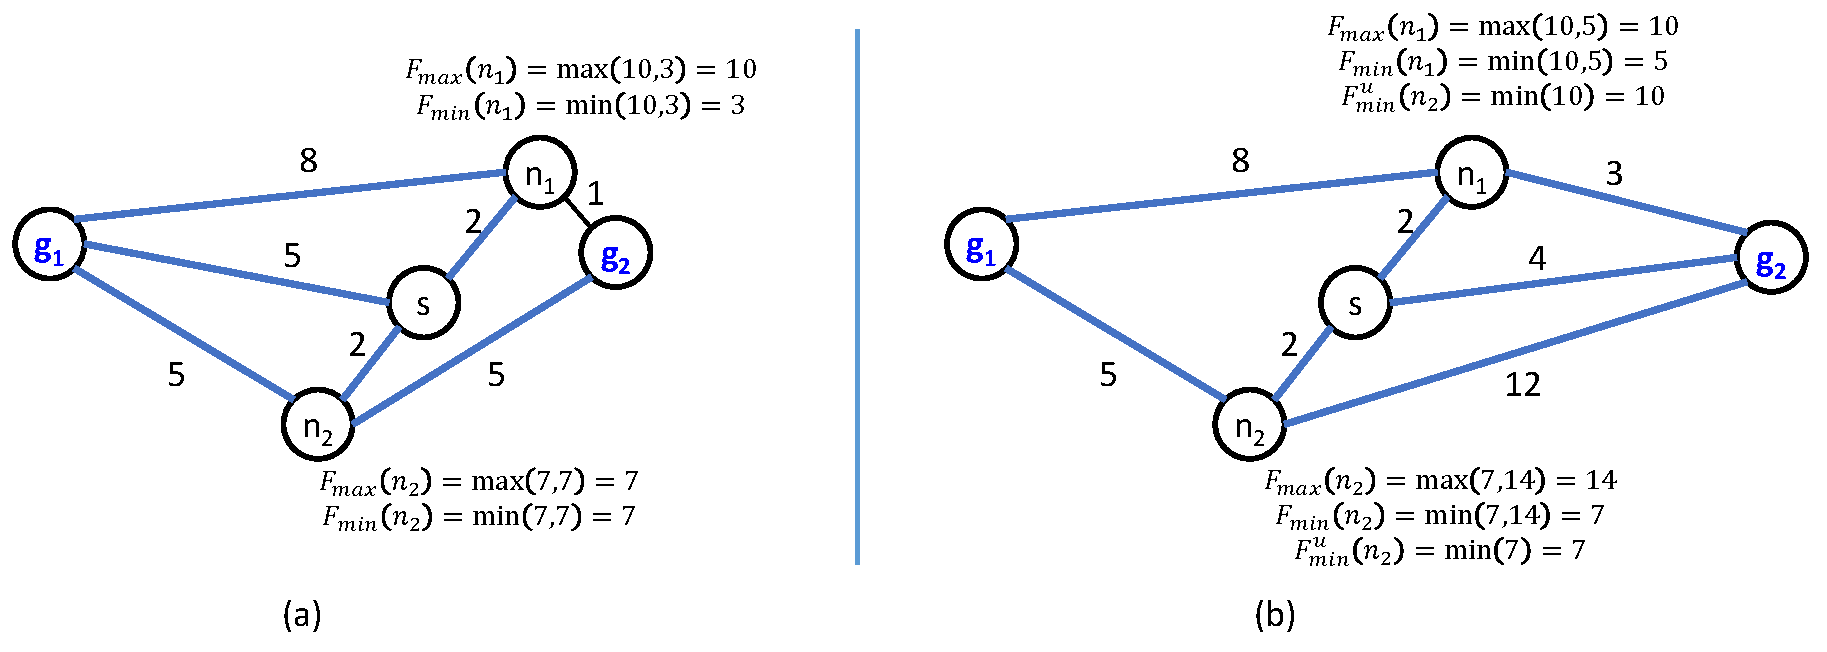
\includegraphics[width=\textwidth]{Lazy_cropped.pdf}      
	\caption{The left hand graph shows an example where using \maxf{} with Lazy \kastar{} results in suboptimal solutions. The right hand graph shows a similar example, but where using Lazy \kastar{} does result in an optimal solutions.}
	\label{fig:lazy}
\end{figure*}

As an example, consider running Lazy \kastar{} with \minf{} on graph depicted in the right hand side of Figure~\ref{fig:lazy}. Assume we have a perfect heuristic in all states except for the goal states $G_1$ and $G_2$ that have a zero heuristic to each other, i.e., $h_2(G_1)=0$ and $h_1(G_2)=0$. After expanding the start state $s$, states $n_1$, $n_2$, and $G_2$ are generated. Using \minf{}, we have $F(n_1)=\max(10,5)=5$, $F(n_2)=\max(7,14)=7$, and $F(G_2)=\max(0,0)=0$. So the next state expanded is goal $G_2$, which is then removed from the set of relevant goals. At this stage, states $n_1$ and $n_2$ are both in \open{} and their $F$ values are {\em stale} in the sense that they were computed for $G_1$ and $G_2$ while the set of relevant goals at this stage contain only $G_2$. According to these stale $F$ values, the next state to choose from \open{} is $n_1$ with $F(n_1)=5$. After popping $n_1$ out of \open{}, however, its $F$ value is re-computed  using Lazy \kastar{}. We denote by $F^u_{min}(n)$ this $F$ value of $n$, which is computed with respect to the current set of relevant states. According to Lazy \kastar{}, if $F^u_{min}(n)\geq F(n)$ then we set $F(n)$ to be $F^u_{min}(n)$ and re-insert $n$ into \open{}. Consequently, $n_2$ will be expanded, followed by $G_1$, finally finding the optimal path to $G_1$ as well. 


% Lazy does not work for Max-f, but does work on Min-f
The correctness of Lazy \kastar{} depends on the node evaluation function. For example, consider running Lazy \kastar{} with \maxf{} on the graph in left hand side of Figure~\ref{fig:lazy}. This is a \kgs{} problem with two goals ($k=2$) that is similar to the example discussed above, and we assume here too that we have the perfect heuristic in all states except for the goal states $G_1$ and $G_2$ that has a zero heuristic to each other ($h_2(G_1)=h_1(G_2)=0$). After expanding the start state $s$, states $n_1$, $n_2$, and $G_1$ are generated. Using \maxf{}, we have $F(n_1)=\max(10,3)=10$, $F(n_2)=\max(7,7)=7$, and $F(G_1)=\max(0,0)=0$. Therefore, $G_1$ is expanded, and is subsequently removed from the set of relevant goals. At this stage, states $n_1$ and $n_2$ are both in \open{} and their $F$ values are {\em stale} in the sense that they were computed for $G_1$ and $G_2$ while the set of relevant goals at this stage contain only $G_2$. According to these stale $F$ values, the next state to expand is $n_2$ with $F(n_2)=7$. This would result in adding $G_2$ to \open{} with $F(G_n)=7$ and subsequently $G_2$ will be expanded and the search will halt, returning a suboptimal path to $G_2$ through $n_2$. If, after $G_1$ was removed from the set of relevant goals the $F$ values of the states in \open{} would have been re-computed and \open{} re-sorted accordingly, then $n_1$ would have been expanded before $n_2$, finding the optimal path to $G_2$. Thus, {\bf using Lazy \kastar{} with \maxf{} is not correct, potentially leading to suboptimal paths to some of the goals}. By contrast, Lazy \kastar{} is correct with \minf{}. 


% Lazy with minf is good
\begin{theorem}[Lazy \kastar{} with \minf{} is admissible]
Every path $\pi_i$ returned by Lazy \kastar{} with \minf{} is guaranteed to be the lowest-cost path to its corresponding goal ($G_i$).
\label{the:lazy-minf-correct}
\end{theorem}
\begin{proof}
	We prove Theorem~\ref{the:lazy-minf-correct} by showing that Lazy \kastar{} with \minf{} and \kastar{} with \minf{} expand exactly the same set of states. For every $n$ it holds that $F_{min}(n)\leq F^u_{min}(n)$, since $F^u_{min}(n)$ is the minimum over a subset of elements that $F_{min}(n)$ is a minimum of. 
	Since it was chosen for expansion then $n$ has the smallest $F$ value in \open{}
	and $F_{min}(n)=F^u_{min}(n)$, i.e., its $F$ value is not stale, as otherwise it would have been re-inserted into \open{}. Therefore 
	\[ \forall n'\in\open{} ~~ F^u_{min}(n)=F_{min}(n)\leq F_{min}(n') \leq F^u_{min}(n') \]
	So, $n$ has the smallest $F^i_{min}$ value in \open{}, and thus it would have also been expanded by \kastar{}. 
\end{proof}

	


%Of course, one may still use Max-$f$ as an anytime algorithm.  Instead of assuming that when expanding a goal the best path to it has been found, we continue the search, , still looking for better path to that goal. The search halted when [[Roni: do we still need to compute the heuristic for these goals?]] [[Roni: What is a good stopping condition for this option?]]
%Concretely, we continued to compute the heuristic for all goals even after they were expanded, thus continuing to guide the search to look for better path continuing the search and looking for better path to the previously expanded goals. 



\section{Runtime Analysis}
% Analysis
In this section we compare analytically the two main approaches we proposed for the \kgs{} problem: $k$ searches for one goal (running \astar{} $k$ times) or one search for $k$-goals (running \kastar{} once). 
In this analysis we will assume that \kastar{} is implemented by eagerly re-sorting \open{} whenever a goal is found, to make the analysis simpler. 



We will focus our analysis on 





Now, we compare the two approaches described above -- $k$ separate SPP problems or one BFS to return all the $k$ paths. 
It is common to estimate the runtime of BFS by counting the number of nodes that are expanded until the goal is found. However, we can show that both approaches will expand the same set of nodes.  However, the computation done per node is different. 

[[Here will come Ariel's analysis of the runtime]]

\subsection{Optimally Effective}
One of the well-known properties of \astar{} is that it is {\em optimally effective}~\cite{dechter}. Informally, this means that given an admissible heuristic $h$, \astar{} will expand no more nodes than any other best-first search
that uses the same heuristic function, up to tie breaking. 
A more recent generalization of \astar{} also provides a similar guarantee
with respect to the number of nodes generated~\cite{Goldenberg}. 
In this section we ask whether we can say something similar about the proposed
best-first search for \kgs{}. 

\begin{definition}[Surplus Nodes and Necessary nodes]
A node $n$ is called a surplus node if $g(n)+h(n)>opt$, where $opt$ is the cost of the lowest cost path. 
A node $n$ is called a necessary node if $g(n)+h(n)<opt$, where $opt$ is the cost of the lowest cost path. 
In the contest of the \kgs{} problem, we say that a node $n$ is a surlpus node for goal $G_i$ if $g(n)+h_i(n)>opt_i$, where $opt_i$ is the cost of hte lowest cost path to $G_i$ (from the initial state). Similarly, $n$ is a necessary node for $G_i$
if $g(n)+h_i(n)<opt_i$. 
\end{definition}
It is know that an \astar{} search using $h_i$ 
must expand all necessary nodes and will not expand any surplus node. 


\begin{lemma}
\kgbfs{} with the Min-$f$ evaluation function never expands a node
that is a surplus node for all goals. 
\label{lem:min-f-no-surplus}
\end{lemma}
The consequene of Lemma~\ref{lem:min-f-no-surplus} is 
that \kgbfs{} with the Min-$f$ evaluation function expands no more nodes
than running $k$ \astar{} searches, up to tie breaking. This suggests towards the 
effectiveness of $kgbfs{}$. Interestingly, this property does not hold when using
the Max-$f$ evaluation function. To show this, consider a \kgs{} problem with two goals 
$G_1$ and $G_2$ (i.e., $k=2$). Now, assume that $opt_1=opt_2=2$
and that the open list has three nodes $n_1, n_2,$ and $n_3$, such that
their $g$ values is one, and the $h_1$ values of $n_1, n_2,$ and $n_3$
are $9,5,$ and $1$, respectively, and the $h_2$ values of $n_1, n_2,$ and $n_3$ 
are $1,5,$ and $9$ respectively. Consequently, the $f$ value for $n_1, n_2,$ and $n_3$
when using Max-$f$ are $10,6,$ and $10$, respectively. Thus, node $n_2$ will be expanded
while it is a surplus node for $G_1$ and for $G_2$. 





\section{Experimental Results}
[[Here will come experimental results]]

\subsection*{Related work}

There are several well-studied graph problems that are related to $k$-goal search. In the traveling salesman problem (TSP), we aim to find a shortest path that passes through a set of vertices. 
...

In multi-objective search, we have multiple objectives function that we wish to optimize. E.g., in a navigation application one may want to optimize for path length and also for ease of navigation. An optimal 
solution to a multi-objective optimization problem is usually a solution that is Pareto-optimal, and it is often the case that one would like the set of all Pareto-optimal solutions. 


An important distinction to make is that \kgs\ is different from the problem where $k$ possible goals are given and the task is to find the shortest path to the closest goal. In \kgs\ we must find the shortest path to each of the goals, and not just to the closest one. 



\section{Conclusion and Future Work}



In future work we will explore ways in which the search for one goal 
can provide information to help searching for the other goals. 

One way to do so in undirected graphs is to use the heuristic for one goal and the 
heuristic between the goals as an admissible heurstic, thus allowing to save the computational cost of re-computing the heuristic of a state if it is generated again for the other goal. This idea is inspired from the canonical heuristics used by path finding algorithms~\cite{canonical}.



% \begin{figure}[!htbp]
%   \centering
%   \includegraphics[width=1\hsize]{filename.eps}
%   \caption{caption} \label{fig:label}
% \end{figure}

\section*{Acknowledgements}
Thanks!

\bibliographystyle{abbrv}
\bibliography{library}

\end{document}
